\documentclass[a4paper]{article}

\usepackage[utf8]{inputenc}
\usepackage[T1]{fontenc}
\usepackage{textcomp}
\usepackage[english]{babel}
\usepackage{amsmath, amssymb}
\usepackage{physics}
\usepackage{isomath}
\usepackage{listings}


% figure support
\usepackage{import}
\usepackage{xifthen}
\pdfminorversion=7
\usepackage{pdfpages}
\usepackage{transparent}
\newcommand{\incfig}[1]{%
	\def\svgwidth{\columnwidth}
	\import{./figures/}{#1.pdf_tex}
}

\DeclareMathSymbol{\C}{\mathalpha}{AMSb}{"43}
\DeclareMathSymbol{\R}{\mathalpha}{AMSb}{"52}

\pdfsuppresswarningpagegroup=1
\title{EE 636 - Matrix Computations}
\begin{document}
\section{Introduction}
The following are course notes made during the live lectures of
EE 636, taken by Prof. Debasattam Pal (Spring 2021)
\textbf{Logistics}
\begin{itemize}
	\item Google Classroom - join codes shared on Moodle
	\item login to classroom regularly to check for assignments, announcements
	\item live lectures
	\item do not rely on the lectures being recorded
\end{itemize}
\textbf{Reference books}
\begin{itemize}
	\item David Watkins - Matrix Computations (Main)
	\item Golub - Matrix Compuations
\end{itemize}
\textbf{Grading Policy}
\begin{itemize}
	\item TA Proctored quizes - 20\%
	\item Midsem - 20\%
	\item Endsem - 40\%
	\item Assignments - 10\%
	\item TakeHomeExam/viva/project/coding - 10\%
\end{itemize}

Take home exams will be significantly harder than assignments, which
will be standard problems. Deadlines will be stricter for take-home-exams.

Learning more about HPC in specific will require you to look into
topics that are beyond the scope of the course, but are in the
reference book.

As such the main aim of this course is to learn what happens behind
the scenes when we call library functions and learn how to write
better code. \textbf{It is important that we understand when the result
of a computation can be trusted or not.} We will see when a computer
is prone to make errors. It has something to do with the condition 
number of the matrix.

Condition number is defined as
\[
	K_2(A) = {\norm{A}_2}{\norm{A^{-1}}_2}
.\] 

We will spend a lot of time seeing how to solve $Ax = b$. We might
not look at specific examples, but the content covered will apply
more or less directly in some use cases e.g. image processing.

Starting off with a small simple assignment, to be submitted before
the next lecture.
\textbf{Assignment}
\begin{itemize}
	\item Go through the syllabus
	\item Write briefly about a problem (from your area of expertise) that needs knowledge from any of the syllabus topics
	\item Feel free to come up with multiple examples. The more examples $\implies$ more credits.
	\item Submission due by next Monday (11th Jan)
	\item To be submitted on the classroom
	\item submission format \texttt{.pdf}
\end{itemize}

Professor asked us here what exactly are we looking for in this course.
Some answers were given by students. The main purpose of this course
is to understand what happens behind the scenes when we call linalg
library functions, and consequently understand whether a particular
computation is trustworthy or not.

\subsection{Types of Problems in Matrix Computations}
%%%%% TODO: reformat, resolve TODOs.
\subsubsection{$\mathrm{A}\vec{x} = \vec{b}$}
where we solve for $x$, where $A \in \mathbb{R}^{m\times n}
		,b \in  \mathbb{R}^{m}
		,x \in \mathbb{R} ^{n}$. Also, note that $\R^{n} = \R^{n\times 1}$.

\subsubsection{$\text{argmin}_{\vec{x}}\norm{\mathrm A \vec{x} - \vec{b}}$}
	Sometimes we cannot find solve for $\vec{x}$ exactly, in which
	case we would like to minimize some norm of the above kind.
\subsubsection{$\mathrm a \vec{x}= \lambda \vec{x}$}
Here we need to solve for both $\vec{x}$ and $\lambda$. This is a
very important class of problems and also not straightforward. The
characteristic equation to be solved is
\begin{equation}\label{chareq}
	\left| \mathrm A - \lambda \mathbb{1} \right|  = 0
\end{equation}
And then we have the older problem of finding $\vec{x}$, the eigenvectors.
The equation \ref{chareq} is basically finding the roots of a polynomial,
which is very nontrivial ($\because$ in general there is no closed
form for degrees $\ge 5$, as shown by Henry Abel.)

Something called the QR algorithm can find both eigvals and eigvecs
in one shot.

\subsubsection{$\mathrm A \vec{u} = \mathrm \sigma \vec{v}$}
$\mathrm A$ is known, the rest are unknown. And
\begin{align}
	&\vec{u_1}\quad \vec{u_2}\ldots\vec{u_n} \\
	&\vec{v_1}\quad \vec{v_2} \ldots \vec{v_m} \\
	&\vec{u_i}
\end{align}
\begin{itemize}
	\item Singular value decomposition
	\item 
\end{itemize}

Questions that we are concerned with, given some problems
\begin{itemize}
	\item How does a computer solve them?
	\item How trustworthy are the solutions?
	\item How efficient are the algorithms?
\end{itemize}

Something was said about the etymology of the word ``algorithm". The
prof then talks about the Caesar cypher. 

The letter ``E" is used most often in English. If you have a very
large encrypted text, you could find the Caesar cypher key by
finding the most frequent letter in the encrypted text. Pretty neat
huh.

The enigma machine would randomly choose a key every day and the
decoder machine could automatically figure out the key from the
encrypted text.

Let's get down to computations and all. What does a computer do when
you tell it to $\mathrm{A}\vec{x} = \vec{b}$.
 \begin{equation}
	 \begin{bmatrix} a_{11} & a_{12} & a_{13} \ldots &a_{1n} \\
	 a_{21} & a_{22} & a_{23} \ldots &a_{2n}\\
	 \hdotsfor{4} \\
	 a_{m1} & a_{m2} & a_{m 3} \ldots &a_{mn}
 \end{bmatrix} 
 \begin{bmatrix} x_1\\ \vdots\\ x_n \end{bmatrix}
\end{equation}

Internally, it computes something like
\begin{equation}
	\begin{pmatrix} \sum_{i=1}^{n} a_{1i}x_i\\ \vdots\\ \sum_{i=1}^{n} a_{mi}x_i \end{pmatrix}
\end{equation}
%%%% TODO: spent too much time figuring out the matrix snippets. Complete this part

\textbf{Task:} Compute the number of tasks required in matrix vector
multiplication. Here, task means FLOP. So, find the number of FLOP.
Prove that rowwise FLOP $= 2mn$ and columnwise FLOP $= 2mn$ and 
$\mathrm{A}\vdot B$ FLOP $= 2mnp$

\section*{Summary}
The purpose of this course is to 
\begin{itemize}
	\item learn how a computer can solve
the four types of problems mentioned a
	\item Effect of round-off errors 
	\item When can a solution be trusted
	\item FLOPS to measure computation time
	\item Counted the FLOPS for basic matrix multiplication: $2mn$ for a matrix of size $m\times n$ and a vector of dim $n$.
\end{itemize}

\section*{Solvinig a linear system of linear equations}
\subsection*{Triangular Matrix}
\begin{equation}
	\mathrm{A}\vec{x} = \vec{b}
\end{equation}
where $\mathrm A \in \R^{m \times  n}$, $b \in  \R^{n}$. The first
step to learning how to solve such problems is learning about
triangular matrix. Consider the following system with a lower
triangular matrix
\begin{equation}
	%%%%% TODO: Complete
	\begin{bmatrix} l_{11} & 0 & 0 & \ldots & 0\\
		l_{21} & l_{22} & 0 & \ldots & 0 \\
		l_{31} & l_{32} & l_{33} & \ldots & 0\\
	\hdotsfor{5} \\  
	l_{n 1} & l_{n 2} & l_{n 3} &\ldots & l_{nm} \end{bmatrix}
%	\begin{bmatrix}  \end{bmatrix} %%%% TODO
\end{equation}

\lstinputlisting{listings/ltr.c}

For the above algorithm (\emph{forward substitution}), FLOPS $= n(n-1) + n = n^2$.
Innermost loop has $2(k-1)$ FLOPS. The loop is called $n$ times for
$k = 1,2,\ldots n$. There is another division operation after a whole
pass over the the inner loop. So, we have $n + \sum_{j=1}^{n} a_n z^n$ TODO. %%% TODO

In general, we can have a column-oriented algorithm for a row-oriented
operation. The corresponding algo is called \emph{backward substitution}. 
FLOPs will be the same as the row-oriented business.

\subsection*{The question of solvability}
In real life we do not really get such nice looking lower-triangular
or upper triangular matrices. Consider the following theorem

\textbf{Theorem:} Let $\mathrm A \in \R^{n\times n}$ and $b \in  \R^{n}$ be given. Then the following are equivalent
\begin{enumerate}
	\item $\mathrm A \vec{x}= \vec{b}$ has a unique solution
	\item $\mathrm A^{-1}$ exists
	\item $\text{det} A \neq 0$ 
	\item The rows of $\mathrm A$ are linearly independent
	\item The columns are linearly independent
	\item $\mathrm A\vec{y} = 0 \iff y = 0$
\end{enumerate}
How do we prove $1 \implies 2$? (Notation: $\vec{e_i}$ are the unit vectors).
$\vec{b} = \sum_{j=1}^{n} a_j\vec{e_j}$ And $\vec{x} = \sum_{j=1}^{n} x_i \vec{e_i}$

\[
	\mathrm A \vec{x} = \sum_{i=1}^{n} x_i \mathrm{A}\vec{e_i}
.\] 
LOL IDK what I am doing. %%%% TODO: write full proof

\subsection*{Gaussian Elimination}
You know what Guassian elimination is from MA 214. Summarizing
na\"ive Gaussian elimination here. We use elementary transformation
$\mathrm{E}$ to reduce $\mathrm{A}$ to an upper triangular form
and solve then use backward substitution.

\begin{equation}
	\label{step_1}
	\begin{split}
	\begin{bmatrix} 
	1 & 0 & 0 & \ldots & 0\\
	-m_{21} & 1 & 0 & \ldots & 0\\
	-m_{31} & 0 & 1 & \ldots & 0 \\
	\hdotsfor{5}\\
	-m_{n 1} & 0 & 0 & \ldots & 1\end{bmatrix}
	\begin{bmatrix}
	a_{11} & a_{12} & a_{13} & \ldots & a_{1n}\\
	a_{21} & a_{22} & a_{23} & \ldots & a_{2n}\\
	a_{31} & a_{32} & a_{33} & \ldots & a_{3 n}\\
	\hdotsfor{5}\\
	a_{n_1} & a_{n 2} & a_{n 3} & \ldots & a_{n n}\end{bmatrix} \\
	= \begin{bmatrix} 
	a_{11} & a_{12} & a_{13} & \ldots & a_{1 n}\\
	0 & a_{22}^{(1)} & a_{23}^{(1)} & \ldots & a_{2 n}^{(1)}\\
	0 & a_{32}^{(1)} & a_{33}^{(1)} & \ldots a_{3 n}^{(1)}\\
	\hdotsfor{5}\\
	0 & a_{n2}^{(1)} & a_{n 3}^{(1)} &\ldots & a_{n n}^{(1)}
\end{bmatrix}
	\end{split}
\end{equation}
where
\begin{equation}
	m_{j 1} = \frac{a_{j1}}{a_{1 1}}, \quad a_{j 1} \neq  0
\end{equation}

This completes one step of procuring an upper triangular matrix. The
next step proceeds by pre-multiplying a similar elementary transformation
matrix to equation (\ref{step_1})
\begin{equation}
	\label{step_2}
	\begin{split}
		\begin{bmatrix} 
	1 & 0 & 0 & \ldots & 0\\
0 & 1 & 0 & \ldots & 0\\
0 & -m_{32} & 1 & \ldots & 0\\
\hdotsfor{5}\\
0 & -m_{n 2} & 0 & \ldots & 1
\end{bmatrix}
\begin{bmatrix}  
	a_{11} & a_{12} & a_{13} & \ldots & a_{1 n} \\
	0 & a_{22}^{(1)} & a_{23}^{(1)} & \ldots & a_{2 n}^{(1)}\\
	0 & a_{32}^{(1)} & a_{33}^{(1)} & \ldots & a_{3 n}^{(1)}\\
	\hdotsfor{5}\\
	0 & a_{n 2}^{(1)} & a_{n 3}^{(1)} & \ldots & a_{n n}^{(1)} 
\end{bmatrix} 	\\
= \begin{bmatrix} 
	a_{11} & a_{21} & a_{13} & \ldots & a_{1 n} \\
0 & a_{22}^{(1)} & a_{23}^{(1)} & \ldots & a_{2n}^{(1)}\\
0 & 0 & a_{33}^{(2)} & \ldots & a_{3 n}^{(2)}\\
\hdotsfor{5}\\
0 & 0 & a_{n 3}^{(2)} & \ldots & a_{n n}^{(2)}\end{bmatrix} ,
	\end{split}
\end{equation}
where
\begin{equation}
	m_{j 2} = \frac{a_{j2}^{(1)}}{a_{2 2}^{(1)}}.
\end{equation}

You can see the upper triangular matrix forming. In general, we
have 
\begin{equation}
	\label{mij}
	m_{ij} = \frac{a_{ij}^{(j-1)}}{a_{jj}^{(j-1)}}.
\end{equation}

So, Gaussian elimination is basically the process
\begin{equation}
	E_{n-1}E_{n-2}\ldots E_2E_1A = \overline{A}
\end{equation}
where $\overline{A}$ is an upper-triangular matrix. The product
$E_{n -1}E_{n-2}\ldots E_2E_1$ ends up being an upper triangular matrix.

\subsubsection*{When can we proceed with Gaussian elimination?}
Of course, we would like to have $a_{jj}^{(j-1)}$ is non-zero.
Else there will be singularieites as seen in (\ref{mij}).

Of course, checking those values after each step sounds
very inefficient. An equivalent condition is - given $A$, we check
if all of $A_1, A_2, \ldots, A_{n}$ are all invertible, where
\[
	A_k = A(1:k, 1:k)
\] 
is the $k\times k$ upper left submatrix of $A$. Formal proof ditch,
we could look at some informal arguments. Consider  $ k = 1$.
$A_1$ is invertible $\implies a_{11} \neq  0$. This could be our base
case.

Now, the most important point here is that $\text{det}A_k \forall k$ 
is invariant under elementary transformations.
At step $j$, we already have the upper left $k-1 \times  k-1$ matrix
is upper triangular. It can be easily shown that the next elementary
operation would create a $j \times  j$ upper triangular matrix.

Also, the 

\subsection*{Brief Recap\ldots}
Working with a real system
\begin{equation}
    (A + \delta A)x = b + \delta b 
\end{equation}

The numerical solution has some error $\delta x$, with bounds given
by

\begin{equation}
    \frac{\norm{\delta x}}{\norm{x}} \le \ldots
\end{equation}  

The larger the condition number, the closer it is to being a singular
matrice and inversion is numerically unstable. Geometrically, solving
$Ax = b$ is finding the intersection of planes. If the planes are
nearly parallel to each other, then even small deviations in the
planes will lead to large deviations in the intersection point.

\section*{Finite Precision Arithmetic}
Even if we know any quantity with infinite precision, we can only
store a representation of the quantity up to some finite precision.

The computers that use store finite precision binary representations,
and computations of non-discrete systems are typically done using
floating point numbers. A typical floating point representation
is something that looks like this
\begin{equation}
    \label{float-rep}
    x_1\vdot x_2x_3x_4x_5 \times 10^{y_1y_2}
\end{equation}

Where $x_i$ are the digits in some base. Computers use binary, i.e.
base 2. In general, there can be multiple representations that
we can work with in computers. There was a need for standardization.
So, most machines follow the IEEE standard.

\subsection*{IEEE 754}
In (\ref{float-rep}), the $x$ part is called the mantissa, and the
 $y$ part is called the exponent. Typically there is also a sign bit.
Per IEEE 754, single precision, typically implemented as a 32 bit
word representation.
\begin{itemize}
    \item 24 significand bits, including sign bit
    \item 8 exponent bits, with a bias of 127
\end{itemize}

In general, any floating point number (other than 0.0) can be
represented as $1.x_1x_2x_3\ldots \times 10\text{e}y_1y_2\ldots$
In the IEEE representation, the $1.$ is implicit and only the
digits after the decimal are stored. This results in a somewhat
quirky represenation of 0.0.

\begin{figure}[h]
    \centering
    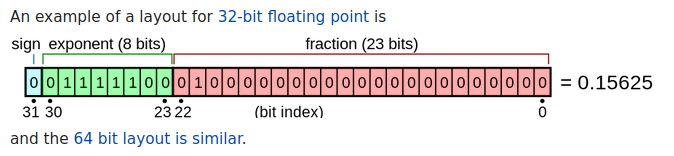
\includegraphics[width=0.8\textwidth]{figures/ieee754_1.png}
    \caption{An example taken from Wikipedia}
    \label{fig:figures-ieee754_1-png}
\end{figure}

So, essentially your real line has been discretized.

\subsection*{Quantization Error}
Given any $x \in  \R$ the computer takes it as $\hat{x}:=fl(x)$,
i.e. converts it to a floating point representation in its word
length.

\begin{equation}
    \hat{x} = \text{fl}(x) = x(1+\epsilon)
\end{equation}

$\epsilon$ is called the per-unit error.

What is the maximum possible error introduced when
converting a real quantity from $\R$ to IEEE 754? It's the
machine epsilon. Assume that the mantissa has $s$ bits. The
machine epsilon is given by
\begin{equation}
    u \approx \frac{1}{2}10^{1-s}
\end{equation}

\subsection*{Operations on Floating Point Numbers}
If you have a binary operator that works with two numbers
from $\R$, you want to be able to simulate it.

Let the `real' operation be $O(x,y)$, where  $x, y \in  \R$.
What the machine sees and does is $F(O(\hat{x},\hat{y}))$,
i.e. some errors will be introduced.
\begin{equation}
    \label{fpop}
    \begin{split}
        R &= F(O(x(1 + \epsilon_1), y(1 + \epsilon_2)))\\
          &= O(x,y)(1 + \epsilon)
    \end{split}
\end{equation}

Let's start with looking at what happens to our basic
arithmetic operations.

\subsubsection*{Multiplication}
\begin{equation}
    \begin{split}
        F(x_1x_2) &= (x_1(1+\epsilon_1)x_2(1 + \epsilon_2))(1 + \epsilon_3)\\
                  &= x_1x_2(1 + \epsilon_1)(1+\epsilon_2)(1+\epsilon_3)\\
                  &= x_1x_2(1 + \epsilon_1 + \epsilon_2
                  + \epsilon_3 + \mathcal{O}(u^3))
    \end{split}
\end{equation}
So, for multiplication the significant error goes as $3u\approx \mathcal{O(u)}$

\subsubsection*{Division}
\begin{equation}
F(\frac{x_1}{x_2}) \approx (\frac{x}{y})(1 + \varepsilon + \mathcal{O}(u^2))
\end{equation}

\subsubsection*{Addition}
This is troublesome
\begin{equation}
    \begin{split}
    F(x_1 + x_2) &= x_1(1 + \epsilon_1) + x_2(1 + \epsilon_2)\\
                 &= (x_1+x_2)(1 + \frac{x_1\epsilon_1}{x_1 + x_2} + \frac{x_2\epsilon_2}{x_1 + x_2})
    \end{split}
\end{equation}
The relative error depends on the operands. So, the error
will blow up if $x + y$ is small. This would happen if
$x$ and $y$ have similar magnitudes, different signs.

E.g. if $x = 1.24456$ and  $y = 1.23421$, so that
 $\hat{x} = 1.2346$ and $\hat{y} = 1.2342$. We have
$\hat{x} - \hat{y} = 0.0004$, while $x - y = 0.00035$.
This is like approximating 35 as 40. 14\% error.
Meanwhile, the truncation errors were some 0.001\%.
Absolutely mad.

This is called catastrophic cancellation.
This error can reach as high as 30\%. Imagine how much
error is introduced in Gaussian elimination. Computer
scientists were aware of the catastrophic cancellation
errors.

The only way around this is to use different numerical
algorithms, i.e. something that uses addition instead of
subtraction, and figure out the upper bounds for errors
in any numerical algorithm before we even start doing
the computation.

\end{document}
